    Наиболее простым видом столкновительно-индуцированных спектров являются трансляционные спектры, порождаемые смесью двух благородных газов при низком давлении, где доминируют бинарные столкновения. При более высоких давлениях будут случаться столкновения с участием трех и более атомов, которые будут видоизменять форму спектра поглощения. На рис. \ref{pic-two-atom-experiment} приведены примеры экспериментальных столкновительно-индуцированных спектров поглощения в дальней ИК области систем He$-$Ar, Ne$-$Ar и Ar$-$Kr \cite{frommhold}. Было экспериментально подтверждено, что интенсивность поглощения линейно зависит от произведения плотностей газов $\rho_1 \rho_2$, что говорит о том, что спектр порождается парами разных атомов. Отклонение от линейной зависимости будет говорить о том, что при данных концентрациях существенный вклад вносят многочастичные столкновения. Спектры, изображенные на рис \ref{pic-two-atom-experiment}, сняты при разных концентрациях от 60 амага (He$-$Ar) до 200 амага (Ar$-$Kr).  

\begin{figure}[H]
    \centering
    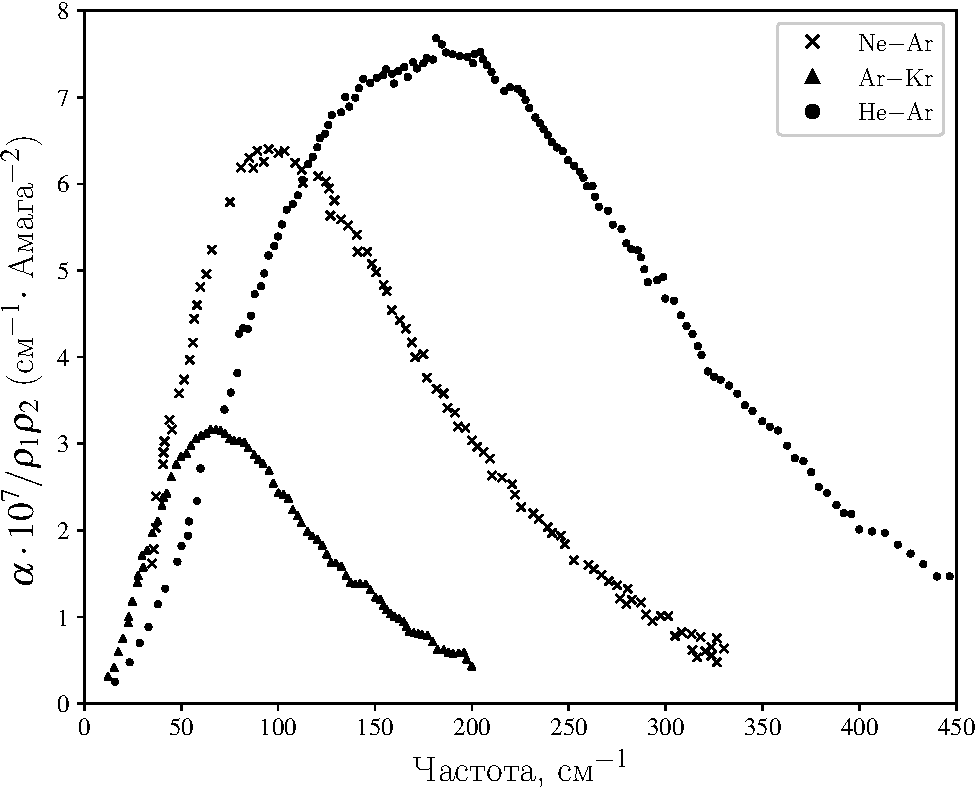
\includegraphics[width=0.7\linewidth]{./pictures/twoatom_experiment/experiment_diatom_spectra-crop.pdf}
    \label{pic-two-atom-experiment}
    \caption{Экспериментальные спектры бинарного поглощения систем гелий$-$аргон, неон$-$аргон и аргон$-$криптон при комнатной температуре \cite{frommhold}}
\end{figure}

В работе \cite{kranendonk1973} авторы разрабатывают формализм расчета столкновительно-индуцированного спектра в приближении бинарных столкновений. Авторы рассматривают систему, состояющую из молекулы $H_2$, возмущенной атомами $Ar$. Вращательное движение молекулы $H_2$ исключено из рассмотрения -- обе сталкивающихся молекулы рассматриваются как безструктурные сферически-симметричные частицы. \par
    Спектральная функция, определяющая профиль спектра поглощения, связана с функцией автокорреляции суммарного дипольного момента системы преобразованием Фурье
\begin{gather}
    J(\omega) = \intty \mean{ \bs{\mu}(0) \bs{\mu}(t) } e^{i \omega t} dt. \label{twoatom-spectral-function}
\end{gather} 
В приближении бинарных столкновений корреляционная функция суммарного дипольного момента становится 
\begin{gather}
    \mean{ \bs{\mu}(0) \bs{\mu}(t) } = N \mean{ \bs{\mu}_1(0) \bs{\mu}_1(t) },
\end{gather} 
%
где через $\bs{\mu_1}(t)$ обозначен дипольный момент индуцированный квадрупольным полем молекулы $H_2$ на атоме $Ar$, а $N$ -- количество рассматриваемых пар. Приведенную массу системы обозначают через $\mu$; вектор, соединяющий центр масс молекулы $H_2$ атомом $Ar$ -- через $\mathbf{R}$; потенциал взаимодействия -- через $V(R)$ $[$как уже говорилось, вращательное движение молекулы водорода не рассматривается, поэтому потенциал зависит только от расстояния между центрами масс $R$$]$. Автокорреляционную функцию дипольного момента приводят к виду 
\begin{gather}
    C(\tau) = \frac{N}{V} \lb \frac{\mu}{2 \pi k T} \rb^{3/2} \iint \bs{\mu}_1(\mathbf{R}) \cdot \bs{\mu}_1(\mathbf{R}(\tau)) \exp \lb -\frac{\mu \dot{\mf{R}}^2}{2 k T} \rb g_0(R) \, d \mathbf{R} \, d \dot{\mathbf{R}}, \label{kranendonk-correlation-function}
\end{gather}
%
где $\mathbf{R}(\tau)$ -- значение $\mathbf{R}$, вычисленное в момент времени $\tau$ путем расчета классической траектории, начальными условиями для которой взяты $\mf{R}$ и $\dot{\mf{R}}$, и $g_0(R)$ -- парная функция распределения (вероятность того, что между атомами расстояние $R$)
\begin{gather}
    g_0(R) = \exp \lb -\frac{V(R)}{kT} \rb.
\end{gather}

Выражение \eqref{kranendonk-correlation-function} неудобно для численного расчета, т.к. в нем имеется $R(\tau)$ для произвольного момента времени $\tau$. Для более эффективной вычислительной схемы предлагается переписать интегральное выражение \eqref{kranendonk-correlation-function} как интеграл по полным столкновительным траекториям. При этом будут рассматриваться только траектории рассеяния. В лабораторной системе отсчета энергия система может быть записана в виде
\begin{gather}
    E = \frac{1}{2} \mu \dot{\mf{R}}^2 + V(R).
\end{gather}
Траекторию рассеяния, которая имеет в момент времени $t$ радиус-вектор $\mf{R}$ и скорость $\dot{\mf{R}}$, может быть однозначно определена относительной скоростью $\mf{g}$ в момент времени $t = -\infty$, прицельным параметром $b$, углом, определяющим ориентацию плоскости столковения $\varepsilon$, и моментом времени $t_0$, в которое произошло столкновение. Применяя теорему Лиувилля
\begin{gather}
    d \mf{R} \, d\dot{\mf{R}} = g d(t - t_0) b db \, d\varepsilon \, d\mf{g},
\end{gather}
%
выражение \eqref{kranendonk-correlation-function} преобразуют к виду
\begin{gather}
    C(\tau) = \frac{N}{V} \lb \frac{\mu}{2 \pi k T} \rb^{3/2} \idotsint \bs{\mu}_1(t) \cdot \bs{\mu}_1(t + \tau) \, g \exp \lb - \frac{\mu \mf{g}^2}{2 k T} \rb b \, db \, d\varepsilon \, d \mf{g}. \label{correlation-function-kranendonk}
\end{gather}

Корреляцией двух функций $f$ и $g$, определенных на комплексной плоскости $\mathbb{C}$, называют функцию, определенную следующим интегралом
\begin{gather}
    C(\tau) = \intty f^{*}(t) g(\tau + t) dt,
\end{gather}
% 
где $*$ обозначает комплексное сопряжение. Обозначим через $F(\omega)$, $G(\omega)$ Фурье-образы функций $f(t)$, $g(t)$. Перепишем выражение для корреляции, представив функции через обратное преобразование Фурье от $F(\omega)$, $G(\omega)$, соответственно.
\begin{gather}
    C(\tau) = \intty \lsq \, \intty F^{*}(\omega) e^{-i \omega t} \frac{d \omega}{2 \pi} \rsq \lsq \, \intty G(\omega^\prime) e^{i \omega^\prime (\tau + t)} \frac{d\omega^\prime}{2 \pi} \rsq
\end{gather}

Осуществляя перестановку внутри интегрального выражения, приходим к следующему выражению 
\begin{gather}
    C(\tau) = \frac{1}{2\pi} \intty \intty F^*(\omega) G(\omega^\prime) e^{i \omega^\prime \tau} \lsq \, \intty e^{i (\omega^\prime - \omega) t} \frac{dt}{2 \pi} \rsq d\omega d\omega^\prime = \notag \\
    = \frac{1}{2\pi} \intty \inty F^*(\omega) G(\omega^\prime) e^{i \omega^\prime \tau} \delta \lb \omega^\prime - \omega \rb d\omega d\omega^\prime = \hat{F}^{-1} \Big[ F^*(\omega) G(\omega) \Big],
\end{gather}
%
где через $\hat{F}$ обозначен оператор преобразования Фурье. Если рассмотреть эту цепочку преобразований для автокорреляционной функции действительной функции $f(t)$, то приходим к теореме Винера-Хинчина \cite{frommhold}
\begin{gather}
    \hat{F} \Big[ C(\tau) \Big] = \Big\vert \hat{F}\Big[ f(t) \Big] \Big\vert^2. 
\end{gather}

Автокорреляционная функция дипольного момента распадается на сумму автокорреляционных функций его компонент
\begin{gather}
    C(\tau) = \intty \bs{\mu}_1(t) \bs{\mu}_1(t + \tau) dt = \sum_{\alpha = x, y, z} \intty \mu_1^\alpha(t) \mu_1^\alpha(t + \tau) dt = C_x(\tau) + C_y(\tau) + C_z(\tau).
\end{gather}

Следовательно, преобразование Фурье от автококорреляционной функции дипольного момента представляет собой сумму квадратов преобразований Фурье от компонент дипольного момента
\begin{gather}
    \hat{F}\Big[ C(\tau) \Big] = \sum_{\alpha = x,y,z} \hat{F} \Big[ C_\alpha(\tau) \Big] = \sum_{\alpha=x,y,z} \Bigg\vert \intty \mu_1^\alpha(t) e^{-i\omega t} dt \Bigg\vert^2,
\end{gather}
% 
что для краткости обозначают 
\begin{gather}
    \hat{F} \Big[ C(\tau) \Big] = \Bigg\vert \intty \bs{\mu}_1(t) e^{-i\omega t} dt \Bigg\vert^2. \label{correlation-theorem}
\end{gather}

Итак, преобразование Фурье от автокорреляционной функции \eqref{correlation-function-kranendonk} дает спектральную функцию  
\begin{gather}
    J(\omega) = \frac{N}{V} \lb \frac{\mu}{2 \pi k T} \rb^{3/2} \idotsint \Bigg\vert \intty \bs{\mu}_1(t) e^{-i \omega t} dt \Bigg\vert^2 \, \exp \lb -\frac{\mu g^2}{2 k T} \rb b \, db \, d \varepsilon \, 4 \pi g^3 dg.
\end{gather}

\section{Cистемы координат для описания движения двух атомов}

Рассмотрим движение двух атомов с массами $m_1$, $m_2$ с радиус - векторами $\mf{r}_1$, $\mf{r}_2$ в поле межатомного потенциала $U(\vert \mf{r}_1 - \mf{r}_2 \vert)$. Задача о движении двух взаимодействующих атомов сводится к задаче о движении виртуальной частицы с приведенной массой $\mu$,  равной 
\begin{gather}
    \mu = \frac{m_1 m_2}{m_1 + m_2}, 
\end{gather}
%
в заданном потенциальном поле $U$ \cite{landau-volume1}. Для описания движения виртуальной частицы введем несколько систем координат. Системой I будем называть декартову систему координат -- положение частицы задается вектором $\mf{r} = \mf{r}_1 - \mf{r}_2$. В этой системе координат лагранжиан и гамильтониан системы записываются как 
\begin{gather}
    \mL_\text{cartesian} = \frac{\mu \dot{\mf{r}}^2}{2} - U( \vert \mf{r} \vert ), \label{two-atom-cartesian-lagrangian} \\
    \mH_\text{cartesian} = \frac{\mf{p}^2}{2\mu} + U( \vert \mf{r} \vert ), \label{two-atom-cartesian-hamiltonian}
\end{gather}
%
где вектор импульса $\mf{p}$ равен
\begin{gather}
    \mf{p} = \frac{\partial \mL_\text{cartesian}}{\partial \dot{\mf{r}}} = \mu \, \dot{\mf{r}}. \label{two-atom-cartesian-momenta}
\end{gather}

Вектор $\mf{r}$ можно представить в сферической системе координат -- длину вектора обозначим через $r$, зенитный и азимутальный углы через $\theta$ и $\varphi$, соответственно ($\theta \in [0, \pi], \phi \in [0, 2 \pi]$. Будем называть эту координатную систему системой II. Лагранжиан и гамильтониан в ней записываются как
\begin{gather}
    \mL_\text{spherical} = \frac{1}{2} \mu \dot{r}^2 + \frac{1}{2} \mu r^2 \dot{\theta}^2 + \frac{1}{2} \mu r^2 \dot{\varphi}^2 \sin^2 \theta - U(r),  \label{two-atom-spherical-lagrangian} \\
    \mH_\text{spherical} = \frac{p_r^2}{2 \mu} + \frac{p_\theta^2}{2 \mu r^2} + \frac{p_\varphi^2}{2 \mu r^2 \sin^2 \theta} + U(r), \label{two-atom-spherical-hamiltonian}
\end{gather}
%
где обобщенные импульсы $p_r$, $p_\theta$, $p_\varphi$ связаны с обобщенными скоростями соотношениями
\begin{gather}
    p_r = \frac{\partial \mL_\text{spherical}}{\partial \dot{r}} = \mu \dot{r}, \quad \dot{r} = \frac{p_r}{mu} \label{two-atom-spherical-momenta1} \\
    p_\theta = \frac{\partial \mL_\text{spherical}}{\partial \dot{\theta}} = \mu r^2 \dot{\theta}, \quad \dot{\theta} = \frac{p_\theta}{\mu r^2} \label{two-atom-spherical-momenta2} \\
    p_\varphi = \frac{\partial \mL_\text{spherical}}{\partial \dot{\varphi}} = \mu r^2 \dot{\varphi} \sin^2 \theta \quad \dot{\phi} = \frac{p_\varphi}{\mu r^2 \sin^2 \theta} \label{two-atom-spherical-momenta3}.
\end{gather}

Декартовы координаты виртуальной частицы связаны со сферическими координатами следующими соотношениями
\begin{gather}
    \lc
    \begin{aligned}
        x &= r \cos \varphi \sin \theta \\
        y &= r \sin \varphi \sin \theta \\
        z &= r \cos \theta
    \end{aligned}
    \right. \label{two-atom-spherical-coordinates}
\end{gather}

Рассмотрим, как связаны декартовы импульсы $\mf{p}$ с импульсами $p_r$, $p_\theta$, $p_\phi$, сопряженными сферическим координатам. Для этого продифференцируем соотношения \eqref{two-atom-spherical-coordinates} по времени и умножим обе части на приведенную массу $\mu$, получив в левой части компоненты вектора $\mf{p}$ согласно \eqref{two-atom-cartesian-momenta}, а в правой части подставим выражения обобщенных скоростей $\dot{r}$, $\dot{\theta}$, $\dot{\varphi}$ через соответствующие импульсы \eqref{two-atom-spherical-momenta1}, \eqref{two-atom-spherical-momenta2}, \eqref{two-atom-spherical-momenta3}
\begin{gather}
    \lc 
    \begin{aligned}
        p_x &= p_r \cos \varphi \sin \theta + \frac{p_\theta}{r} \cos \varphi \cos \theta - \frac{p_\varphi}{r} \frac{\sin \varphi}{\sin \theta} \\ 
        p_y &= p_r \sin \varphi \sin \theta + \frac{p_\theta}{r} \sin \varphi \cos \theta + \frac{p_\varphi}{r} \frac{\cos \varphi}{\sin \theta} \\ 
        p_z &= p_r \cos \theta - \frac{p_\theta}{r} \sin \theta 
    \end{aligned}
    \right. \label{two-atom-cartesian-spherical-momenta}
\end{gather}

Разрешая линейные соотношения \eqref{two-atom-cartesian-spherical-momenta} относительно импульсов $p_r$, $p_\theta$, $p_\varphi$, находим соотношения, выражающие обратную связь импульсов.
\begin{gather}
    \lc
    \begin{aligned}
        p_r &= r \lb p_x \cos \varphi \sin \theta + p_y \sin \varphi \sin \theta + p_z \cos \theta \rb\\
        p_\varphi &= r \sin \theta \lb p_y \cos \varphi - p_x \sin \varphi \rb \\
        p_\theta &= r \lb p_x \cos \varphi \cos \theta + p_y \sin \varphi \cos \theta - p_z \sin \theta \rb  
    \end{aligned}
    \right.
\end{gather}

Выразим компоненты углового момента через координаты и импульсы системы II, пользуясь соотношениями \eqref{two-atom-cartesian-spherical-momenta}
\begin{gather}
    \mf{J} = \lsq \mf{r} \times \mf{p} \rsq = 
    \begin{bmatrix}
        -p_\theta \sin \varphi - p_\varphi \cos \varphi \cot \theta \\
        -p_\varphi \sin \varphi \cot \theta + p_\theta \cos \varphi \\
        p_\varphi
    \end{bmatrix}. \label{two-atom-angular-momenta-spherical} 
\end{gather}

Известно, что в отсутствии внешнего момента сил движение двухатомной системы происходит в плоскости, перпендикулярной вектору углового момента $\mf{J}$ \cite{goldstein}. Следовательно, движение системы можно описать при помощи полярных координат $r, \psi$, определенных в плоскости, и соответствующих обобщенных скоростей $\dot{r}$, $\dot{\psi}$. Ориентацию плоскости будем задавать при помощи пары сферических углов $\Phi$, $\Theta$, описывающих ориентацию вектора углового момента. Определим систему координат таким образом, чтобы координатные оси $OXY$ совпадали с плоскостью движения, а ось $OZ$ была сонаправлена с вектором углового момента $\mf{J}$. Будет называть эту координатную систему системой III; лагранжиан и гамильтониан в ней равны 
\begin{gather}
    \mL_\text{plane} = \frac{1}{2} \mu \dot{r}^2 + \frac{1}{2} \mu r^2 \dot{\psi}^2 - U(r), \label{two-atom-plane-lagrangian} \\
    \mH_\text{plane} = \frac{p_r^2}{2\mu} + \frac{p_\psi^2}{2 \mu r^2} + U(r), \label{two-atom-plane-hamiltonian} 
\end{gather}
%
где обобщенные импульсы $p_r$, $p_\psi$ связаны с обобщенными скоростями следующими соотношениями
\begin{gather}
    p_r = \frac{\partial \mL_\text{plane}}{\partial \dot{r}} = \mu \dot{r}, \quad \dot{r} = \frac{p_r}{\mu} \label{two-atom-plane-momenta1} \\
    p_\psi = \frac{\partial \mL_\text{plane}}{\partial \dot{\psi}} = \mu r^2 \dot{\psi}, \quad \dot{\psi} = \frac{p_\psi}{\mu r^2}.  \label{two-atom-plane-momenta2}
\end{gather}

Перевод полярных координат $r$, $\psi$ системы III в декартовы координаты $\mf{r} = \lc x, y, z \rc$ системы I можно осуществить при помощи ортогональной матрицы вращения $\bbS$, параметризованной углами $\Phi$, $\Theta$ \cite{goldstein} 
\begin{gather}
    \begin{bmatrix}
        x \\ y \\ z
    \end{bmatrix} = \bbS_\Phi^{-1} \bbS_\Theta^{-1} 
    \begin{bmatrix}
        r \cos \psi \\ r \sin \psi \\ 0
    \end{bmatrix}, \label{two-atoms-coordinate-transformation}
\end{gather}
% 
где матрицы поворота $\bbS_\Phi$, $\bbS_\Theta$ определены равны
\begin{gather}
    \bbS_\Phi = 
    \begin{bmatrix}
       -\sin \Phi & \cos \Phi & 0 \\
       -\cos \Phi & -\sin \Phi & 0 \\
      0 & 0 & 1
    \end{bmatrix}, \quad
    \bbS_\Theta = 
    \begin{bmatrix}
        1 & 0 & 0 \\
        0 & \cos \Theta & \sin \Theta \\
        0 & -\sin \Theta & \cos \Theta
    \end{bmatrix}.
\end{gather}

Раскрывая матричное выражение \eqref{two-atoms-coordinate-transformation}, получаем 
\begin{gather}
    \left\{
        \begin{aligned}
            x &= -r \cos \psi \sin \Phi - r \sin \psi \cos \Phi \cos \Theta \\
            y &= r \cos \psi \cos \Phi - r \sin \psi \sin \Phi \cos \Theta \\
            z &= r \sin \psi \sin \Theta
        \end{aligned}
    \right. \label{two-atoms-coordinates-transformation2}
\end{gather}

Продифференцируем соотношения \eqref{two-atoms-coordinates-transformation2} по времени, учитывая, что углы $\Phi$, $\Theta$ от времени не зависят.
\begin{gather}
    \begin{bmatrix} \dot{x} \\ \dot{y} \\ \dot{z} \end{bmatrix} = 
    \bbS_\Phi^{-1} \bbS_\Theta^{-1}
    \begin{bmatrix} 
        \dot{r} \cos \psi - r \dot{\psi} \sin \psi \\
        \dot{r} \sin \psi + r \dot{\psi} \cos \psi \\
        0 
    \end{bmatrix} \\
    \lc
    \begin{aligned}
        \dot{x} &= - \dot{r} \lb \cos \psi \sin \Phi + \sin \psi \cos \Phi \cos \Theta \rb + r \dot{\psi} \lb \sin \psi \sin \Phi - \cos \psi \cos \Phi \cos \Theta \rb \\ 
        \dot{y} &= \dot{r} \lb \cos \psi \cos \Phi - \sin \psi \sin \Phi \sin \Theta \rb - r \dot{\psi} \lb \sin \psi \cos \Phi - \cos \psi \sin \Phi \cos \Theta \rb \\
        \dot{z} &= \dot{r} \sin \psi \sin \Theta + r \dot{\psi} \cos \psi \sin \Theta
    \end{aligned}
\right. \label{two-atoms-coordinates-transformation3}
\end{gather}

При рассмотрении средних значений функций по фазовому пространству нам понадобятся выражения импульсов $\mf{p}$ через импульсы $p_r$, $p_\psi$. При умножении левых частей соотношений \eqref{two-atoms-coordinates-transformation3} на приведенную массу $\mu$ мы получим компоненты вектора $\mf{p}$ (согласно \eqref{two-atom-cartesian-momenta}). Подставив выражения обобщенных скоростей $\dot{r}$, $\dot{\psi}$ через импульсы $p_r$, $p_\psi$ \eqref{two-atom-plane-momenta1}, \eqref{two-atom-plane-momenta2}, получаем
\begin{gather}
    \lc
    \begin{aligned}
        p_x &= -p_r \lb \sin \psi \cos \Phi \cos \Theta + \cos \psi \sin \Phi \rb + \frac{p_\psi}{r} \lb \sin \psi \sin \Phi - \cos \psi \cos \Phi \cos \Theta \rb \\
        p_y &= p_r \lb \cos \psi \cos \Phi - \sin \Psi \sin \Phi \cos \Theta \rb - \frac{p_\psi}{r} \lb \sin \psi \cos \Phi + \cos \psi \sin \Phi \cos \Theta \rb \\
        p_z &= p_r \sin \psi \sin \Theta + \frac{p_\psi}{r} \cos \psi \sin \Theta 
    \end{aligned}
\right. \label{two-atom-momenta-transformation}
\end{gather}

Найдем координаты вектора углового момента через координаты системы III, исходя из определения вектора углового момента 
\begin{gather}
    \mf{J} = \mu \lsq \mf{r} \times \dot{\mf{r}} \rsq = 
    \begin{bmatrix}
        \mu r^2 \dot{\psi} \cos \Phi \sin \Theta \\ 
        \mu r^2 \dot{\psi} \sin \Phi \sin \Theta \\
        \mu r^2 \dot{\psi} \cos \Theta
    \end{bmatrix},
\end{gather}
или, пользуясь соотношением между скоростью $\dot{\psi}$ и импульсом $p_\psi$ \eqref{two-atom-plane-momenta2}, 
\begin{gather}
    \mf{J} = 
    \begin{bmatrix}
        p_\psi \cos \Phi \sin \Theta \\
        p_\psi \sin \Phi \sin \Theta \\
        p_\psi \cos \Theta
    \end{bmatrix}. \label{two-atom-plane-angular-momenta}
\end{gather}

Выражение \eqref{two-atom-plane-angular-momenta} подтверждает, что углы $\Phi$, $\Theta$ действительно являются сферическими углами для вектора углового момента. Кроме того, замечаем, что импульс $p_\psi$ имеет физический смысл модуля вектора углового момента. Этот факт, впрочем, может быть понят из вида гамильтониана \eqref{two-atom-plane-hamiltonian}. При составлении гамильтониана для движения в плоскости мы использовали два интеграла движения -- например, постоянство двух сферических углов, задающих ориентацию вектора углового момента. Координата $\psi$ является циклической для гамильтониана \eqref{two-atom-plane-hamiltonian} из чего следует, что $p_\psi$ является интегралом движения. Поэтому можно предположить, что импульс $p_\psi$ соответствует третьему интегралу движения -- модулю вектора углового момента, что и подтверждает приведенное рассмотрение. \par
    Соотношения \eqref{two-atoms-coordinates-transformation2}, \eqref{two-atoms-coordinates-transformation3} позволяют перейти от координат системы III к координатам системы I.    
    \color{red}{Понадобятся ли все остальные переходы?}
\color{black}{}

\section{Усреднение функций по фазовому пространству в разных системах координат} \label{section:averaging}

Рассмотрим усреднение некоторой функции $f(\mf{r}, \mf{p})$ по фазовому пространству двухатомной системы, где $\mf{r}$, $\mf{p}$ -- векторы декартовых координат и сопряженных импульсов (система I). 
\begin{gather}
    \mean{f} = \idotsint f(\mf{r}, \mf{p}) \exp \lb -\frac{\mH(\mf{r},\mf{p})}{kT} \rb d \mf{r} \, d\mf{p} \label{two-atom-mean}
\end{gather}

Целью нашего рассмотрения будет нахождение выражений, позволяющих производить усреднение функции $f$ по фазовому пространству, пользуясь координатами систем II и III. \par
Рассмотрим систему совокупную систему уравнений \eqref{two-atoms-coordinates-transformation2}, \eqref{two-atom-momenta-transformation} и найдем якобиан замены переменных $\lc x, y, z, p_x, p_y, p_z \rc$ $\rightarrow$ $\lc r, p_r, \psi, p_\psi, \Phi, \Theta \rc$. Ввиду громоздкости выкладки приводить не будем, выражение для якобиана получается следующее
\begin{gather}
    \text{Jac} = \Bigg\vert \frac{\partial \lsq x, y, z, p_x, p_y, p_z \rsq}{\partial \lsq r, p_r, \psi, p_\psi, \Phi, \Theta \rsq} \Bigg\vert = p_\psi \sin \Theta. \label{two-atom-planar-jacobian}
\end{gather}

Итак, среднее значение \eqref{two-atom-mean} в системе координат III записывается как
\begin{gather}
    \mean{ f } = \int\limits_{0}^{\infty} dr \intty dp_r \int\limits_0^{2\pi} d\psi \int\limits_0^\infty p_\psi dp_\psi \int\limits_0^\pi \sin \Theta d\Theta \int\limits_0^{2\pi} d\Phi f(r, \psi, p_r, p_\psi, \Theta, \Phi) \exp \lb -\frac{\mH_\text{plane}}{k T} \rb. \label{two-atom-mean-plane1} 
\end{gather}

Если усредняемая функция $f(r, \psi, p_r, p_\psi, \Theta, \Phi)$ не зависит от углов $\Theta$, $\Phi$, то среднее значение  \eqref{two-atom-mean-plane1} приходит к виду
\begin{gather}
    \mean{ f } = 4 \pi \int\limits_{0}^{\infty} dr \intty dp_r \int\limits_0^{2\pi} d\psi \int\limits_0^\infty p_\psi dp_\psi f(r, \psi, p_r, p_\psi, \Theta, \Phi) \exp \lb -\frac{\mH_\text{plane}}{k T} \rb. \label{two-atom-mean-plane2} 
\end{gather}

Как уже отмечалось ранее, импульс $p_\psi$ имеет физический смысл модуля углового момента, поэтому область интегрирования этого импульса составляет полуось $(0, +\infty)$, в то время как для радиального импульса -- вся прямая $(-\infty, +\infty)$. \par
Аналогично, рассмотрим совокупную систему уравнений \eqref{two-atom-spherical-coordinates}, \eqref{two-atom-cartesian-spherical-momenta} и найдем якобиан замены переменных $\lc x, y, z, p_x, p_y, p_z \rc$ $\rightarrow$ $\lc r, p_r, \varphi, p_\varphi, \theta, p_\theta \rc$. Якобиан оказывается единичным 
\begin{gather}
    \text{Jac} = \Bigg\vert \frac{\partial \lsq x, y, z, p_x, p_y, p_z \rsq}{\partial \lsq r, p_r, \varphi, p_\varphi, \theta, p_\theta \rsq} \Bigg\vert = 1. 
\end{gather}

Таким образом, среднее значение \eqref{two-atom-mean} в системе координат II записывается как
\begin{gather}
    \mean{f} = \int\limits_0^\infty dr \intty dp_r \int\limits_0^{2\pi} d\varphi \intty dp_\varphi \int\limits_0^\pi d\theta \intty dp_\theta f(r, p_r, \varphi, p_\varphi, \theta, p_\theta) \exp \lb -\frac{\mH_\text{spherical}}{k T} \rb. \label{two-atom-mean-spherical}
\end{gather}

\section{Распределения координат и импульсов в фазовом пространстве в разных системах координат в условиях канонического ансамбля}

Рассмотрим вопрос распределения координат и импульсов в фазовом пространстве в системах координат II и III в условиях канонического ансамбля. Функция распределения в фазовом пространстве в условиях канонического ансамбля задана гамильтонианом системы $\mH$ \cite{hill} 
\begin{gather}
    \rho \lb \mf{q}, \mf{p} \rb = \Gamma_0 \exp \lb -\frac{\mH \lb \mf{q}, \mf{p} \rb}{\kb T} \rb,
\end{gather}
% 
где постоянная $\Gamma_0$ определяется из условия нормировки функции распределения
\begin{gather}
    \int \rho \lb \mf{q}, \mf{p} \rb d \mf{q} \, d\mf{p} = 1.
\end{gather}

Рассмотрим распределения угловых координат $\theta, \varphi$ и импульсов $p_r$, $p_\theta$, $p_\varphi$ системы II при фиксированном большом значении межатомного расстояния $r_\text{fixed} \gg 1$. Пренебрежем значением потенциала $U(r_\text{fixed}) \approx 0$ на расстоянии $r_\text{fixed}$. Удобно представить отношение $\mH / \kb T$ в виде трех квадратичных членов $\lc \frac{1}{2} x_j^2 \rc_{j = 1 \dots 3}$
\begin{gather}
    \frac{\mH_\text{spherical}}{\kb T} = \frac{p_r^2}{2 \mu \kb T} + \frac{p_\theta^2}{2 \mu r_\text{fixed}^2 \kb T} + \frac{p_\varphi^2}{2 \mu r_\text{fixed}^2 \kb T \sin^2 \theta} = \frac{1}{2} x_1^2 + \frac{1}{2} x_2^2 + \frac{1}{2} x_3^2, \label{two-atom-spherical-hamiltonian-xs} 
\end{gather}
%
где переменные $x_j$ выражены как
\begin{gather}
    \lc
    \begin{aligned}
        x_1 &= \frac{p_r}{\sqrt{\mu \kb T}} \\
        x_2 &= \frac{p_\theta}{\sqrt{\mu r_\text{fixed}^2 \kb T}} \\
        x_3 &= \frac{p_\varphi}{\sqrt{\mu r_\text{fixed}^2 \kb T \sin^2 \theta}}
    \end{aligned}
\right. \label{two-atom-xs}
\end{gather}

Переписав гамильтониан в виде \eqref{two-atom-spherical-hamiltonian-xs}, мы видим, что вероятность нахождения системы в элементе фазового объема $d\theta d\varphi dx_1 dx_2 dx_3$ пропорциональна произведению 
\begin{gather}
    \rho \lb \theta, \varphi, x_1, x_2, x_3 \rb \propto \rho_1(x_1) \rho_1(x_2) \rho_1(x_3) \sin \theta, \label{two-atom-xs-phase-element}
\end{gather}
%
где случайные величины $x_j$ распределены по нормальному закону
\begin{gather}
    \rho_1 (x_j) = \frac{1}{\sqrt{2 \pi}} \exp \lb -\frac{x_j^2}{2} \rb. 
\end{gather}

Соотношения \eqref{two-atom-xs} позволяют установить следующие функции распределения для двух импульсов
\begin{gather}
    \lc
    \begin{aligned}
        p_r &\sim \mN \lb 0, \mu \kb T \rb \\
        p_\theta &\sim \mN \lb 0, \mu r_\text{fixed}^2 \kb T \rb 
    \end{aligned},
    \right.
\end{gather}
%
где через $\mN \lb \mu, \sigma^2 \rb$ обозначено нормальное распределение со математическим ожиданием $\mu$ и дисперсией $\sigma^2$. Импульс $p_\varphi$ представляет собой произведение двух случайных величин
\begin{gather}
    p_\varphi = \tilde{x}_3 \cdot \sin \Theta, \label{two-atom-pvarphi-generation}
\end{gather}
% 
где величина $\tilde{x}_3$ распределена по нормальному распределению $\mN \lb 0, \mu \kb T \rb$, а случайная величина $\Theta$ в силу \eqref{two-atom-xs-phase-element} распределена равномерно с косинусом, т.е. плотность распределения по углу $\Theta$ равна 
\begin{gather}
    \rho(\Theta) = \frac{1}{2} \sin \Theta.
\end{gather}

Численная генерация $p_\varphi$ легко осуществляется по выражению \eqref{two-atom-pvarphi-generation}, однако интересно получить аналитическое выражение для плотности распределения, так как похожие распределения возникают при рассмотрении импульсов в многоатомных ван-дер-Ваальсовых комплексах. Получим плотность распределение случайной величины $\sin \Theta$, используя факт, что имеет $\cos \Theta$  равномерное распределение. Очевидно, что на интервале $\lsq 0, \pi \rsq$ знак $\sin \Theta$ определен однозначно, поэтому воспользуемся формулой
\begin{gather}
    \sin \Theta = \sqrt{ 1 - \cos^2 \Theta}.
\end{gather}
Воспользуемся формулой преобразования случайной величины $Y = g(X)$
\begin{gather}
    \rho_Y(y) = \Big\vert \frac{d}{dy} g^{-1}(y) \Big\vert \cdot \rho_X(g^{-1}(y)), \label{distribution-change}
\end{gather}
%
где через $\rho_X(x)$, $\rho_Y(y)$ обозначены плотности случайных величин $X$, $Y$, соответственно. Подставив $g(x) = \sqrt{1 - x^2}$ в \eqref{distribution-change}, получаем следующую плотность распределения величины $\sin \Theta$
\begin{gather}
    \rho_{\sin \Theta}(x) = \frac{x}{\sqrt{1 - x^2}} \cdot \bbI\lsq 0, 1\rsq,
\end{gather}
% 
где через $\bbI\lsq 0, 1 \rsq$ обозначена индикаторная функция, ограничивающая носитель функции отрезком $\lsq 0, 1 \rsq$. Отметим, что полученное распределение является частным случаем распределения Кумарасвами с параметрами $a = 2$, $b = 1/2$. \par
Плотность распределения $\rho_{p_\varphi}$ может быть получена по стандартной формуле плотности случайной величины, являющейся произведением двух других случайных величин
\begin{gather}
    \rho_{p_\varphi}(z) = \intty \rho_{x_3}(z/x) \rho_{\sin \Theta}(x) \frac{dx}{\vert x \vert}.
\end{gather}
Подставив явные выражения для плотностей распределения, получаем следующий интеграл
\begin{gather}
    \rho_{p_\varphi}(z) = \frac{1}{\sqrt{2 \pi}} \int\limits_0^1 \frac{\displaystyle \exp \lb -\frac{z^2}{2x^2} \rb}{\sqrt{1 - x^2}} dx,
\end{gather}
%
разрешив который приходим к
\begin{gather}
    \rho_{p_\varphi}(z) = \frac{\pi}{8} \lb 1 - \text{sgn}(z) \erf \lb \frac{z}{\sqrt{2}} \rb \rb.
\end{gather}
Т.к. угол $\varphi$ не входит в гамильтониан $\mH_\text{spherical}$, то он распределен с равномерной плотностью на отрезке $\lsq 0, 2 \pi \rsq$.

\begin{figure}[H]
    \centering
    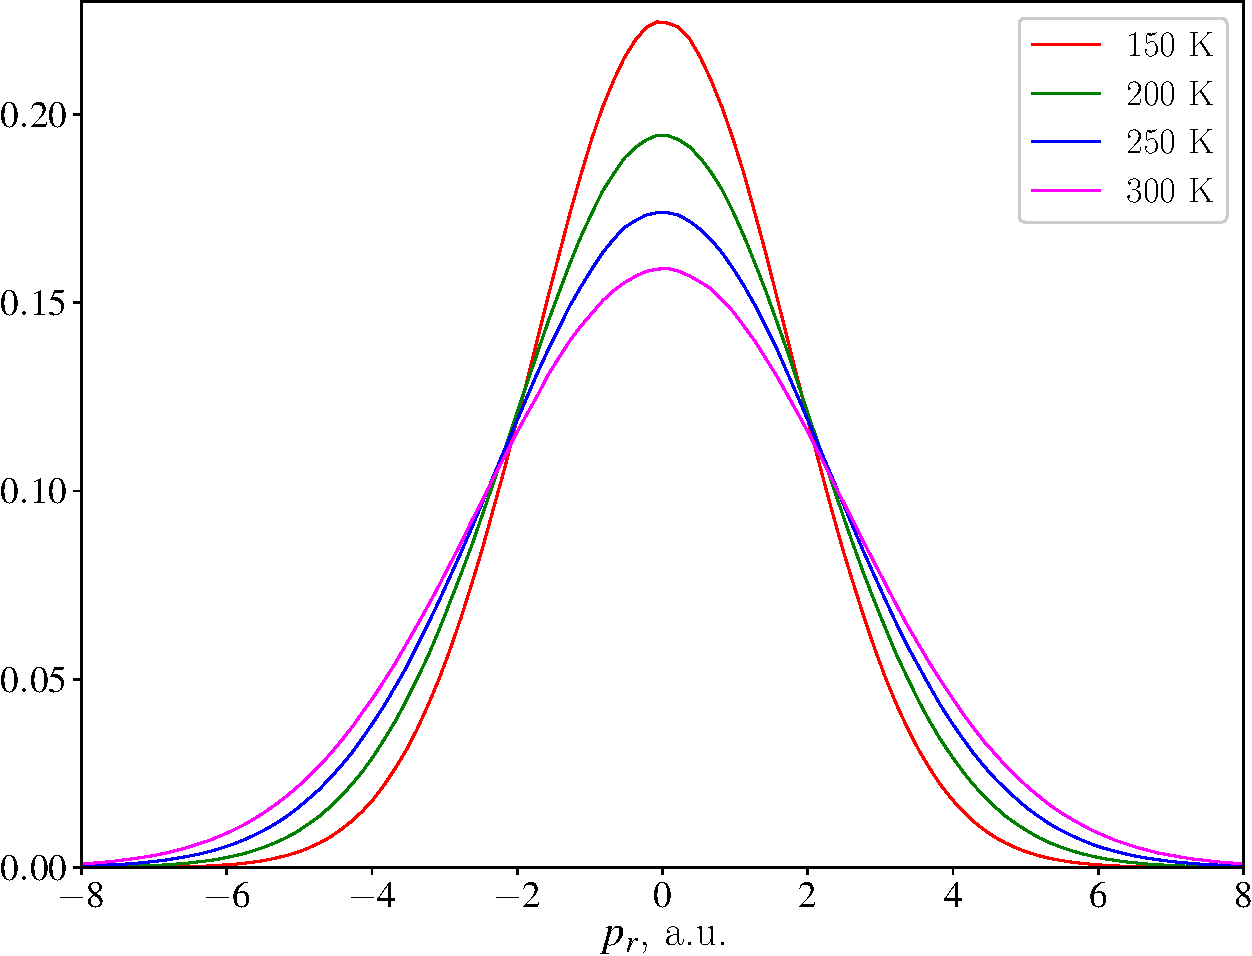
\includegraphics[width=0.75\linewidth]{./pictures/two_atom_distributions/pR-crop.pdf} \\
    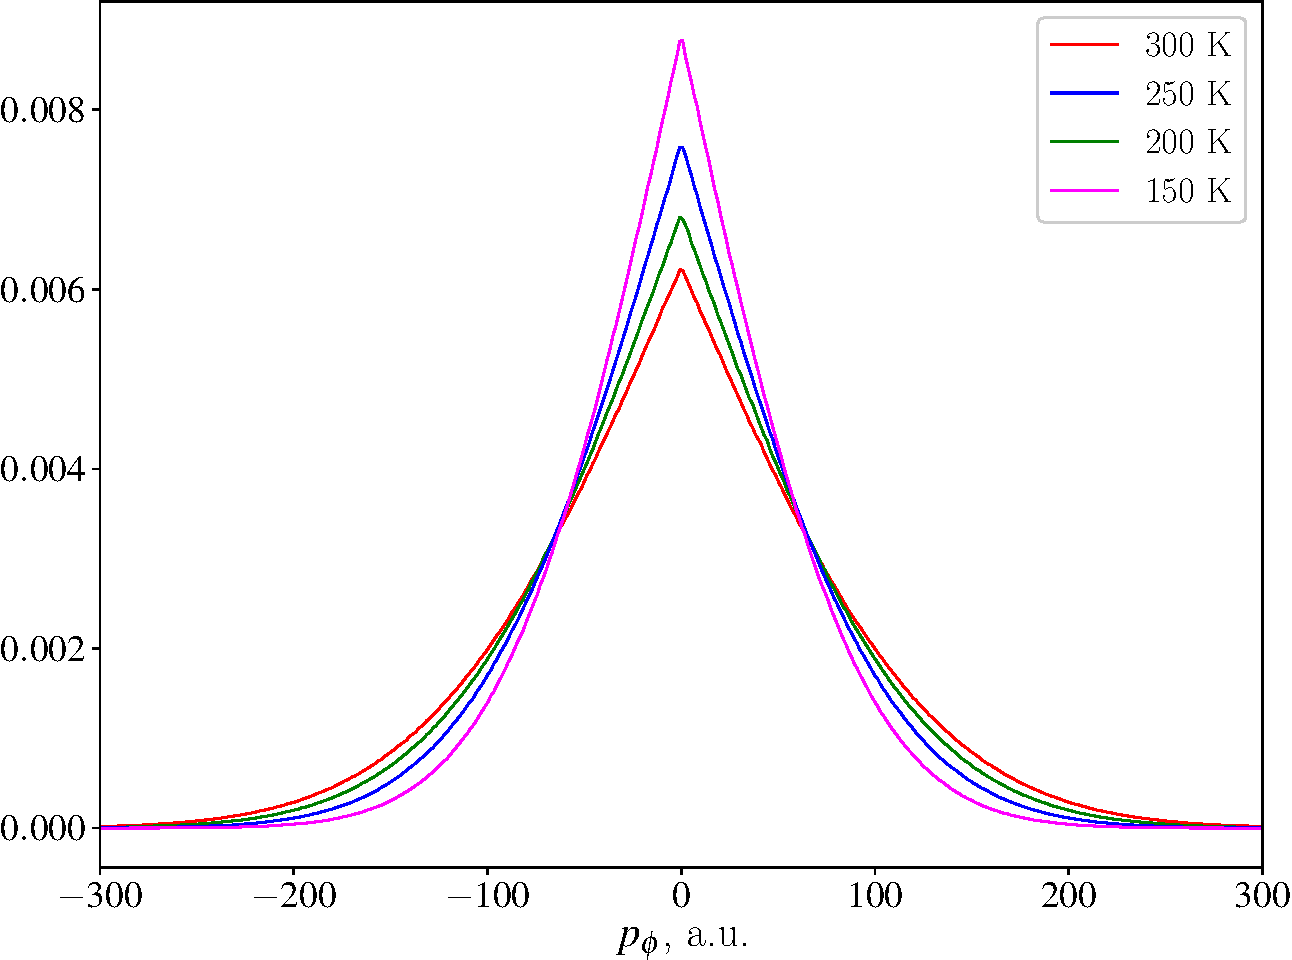
\includegraphics[width=0.75\linewidth]{./pictures/two_atom_distributions/pPhi-crop.pdf}
    \caption{Плотности распределений импульсов $p_r$ и $p_\varphi$ при температурах от 150K до 300K для системы He$-$Ar. Межатомное расстояние $r_\text{fixed}$ взято равным $40 a_0$. Количество сгенерированых точек при каждой температуре -- $N = 5 \cdot 10^7$.}
\end{figure}

Если переходить теперь к переменным системы координат III, то легко заметить, что плотность распределения импульса $p_r$ совпадает с той, что была получена в системе координат II. Угол $\psi$ не входит в гамильтониан, следовательно распределен с равномерной плотностью. Т.к. якобиан замены декартовых координат и импульсов на координаты и импульсы системы III равен $p_\psi \sin \Theta$ (соотношение, следовательно распределен с равномерной плотностью. Т.к. якобиан замены декартовых координат и импульсов на координаты и импульсы системы III равен $p_\psi \sin \Theta$ (соотношение \eqref{two-atom-planar-jacobian}), то получаем, что плотность распределения импульса $p_\psi$ пропорциональна
\begin{gather}
    \rho(p_\psi) \propto p_\psi \exp \lb -\frac{p_\psi^2}{2 \mu r_\text{fixed}^2 \kb T} \rb, \label{two-atom-ppsi-distribution}
\end{gather}
где константа пропорциональна устанавливается из условия нормировки, оказывается равной $1/(\mu r_\text{fixed}^2 \kb T)$. Из того же якобиана замечаем, что угол $\Theta$ распределен равномерно с косинусом. \par
Распределение для импульса $p_\psi$ может быть установлено и из других соображений. Как уже отмечалось, $p_\psi$ имеет физический смысл модуля углового момента $\mf{J}$. Исходя из выражения \eqref{two-atom-angular-momenta-spherical} получаем, что квадрат модуля углового момента $J^2$ связан с импульсами $p_\varphi$, $p_\theta$ соотношением
\begin{gather}
    J^2 = p_\psi^2 = p_\theta^2 + \frac{p_\varphi^2}{\sin^2 \theta}. \label{two-atom-angular-momenta-connection} 
\end{gather}
Мы уже установили, что слагаемых в правой части \eqref{two-atom-angular-momenta-connection} распределены согласно нормальному распределению. Квадраты нормально распределенных случайных величин распределены согласно хи-квадрат распределению с одной степенью свободы $\chi_1^2$ \cite{castaneda}. А сумма двух одномерных хи-квадрат распределений $\chi_1^2$ дает двумерное хи-квадрат распределение $\chi_2^2$. Наконец, для того, чтобы получить распределение величины $p_\psi$, извлекаем корень из двумерного хи-квадрат распределения $\chi_2^2$ и получаем двумерное хи-распределение $\chi_2$, известное как распределение Рэлея, плотность которого задается  
\begin{gather}
    \rho(x; \sigma) = \frac{x}{\sigma^2} \exp \lb -\frac{x^2}{2 \sigma^2} \rb. \label{rayleigh-density}
\end{gather}

Выражение \eqref{two-atom-ppsi-distribution} является частным случаем \eqref{rayleigh-density} с $\sigma^2 = \mu r_\text{fixed}^2 \kb T$.

\begin{figure}[H]
    \centering
    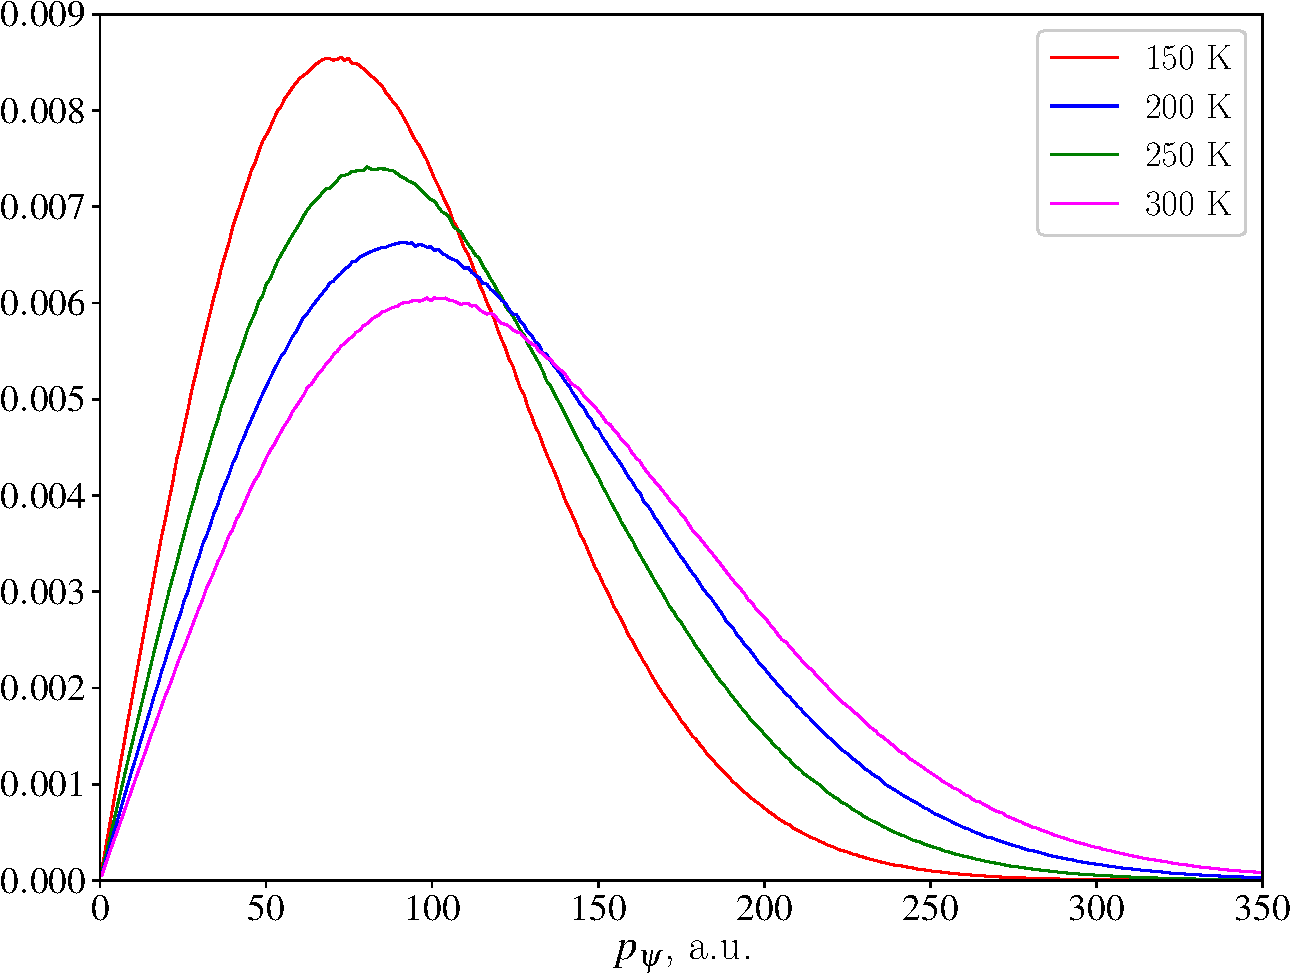
\includegraphics[width=0.75\linewidth]{./pictures/two_atom_distributions/pPsi-crop.pdf}
    \caption{Плотности распределений импульса $p_\psi$ при температурах от 150К до 300К для системы He$-$Ar. Межатомное расстояние $r_\text{fixed}$ было взято равным $40a_0$. Количество сгенерированных точек при каждой температуре -- $N = 5 \cdot 10^7$.}
\end{figure}

\section{Спектральная функция при рассмотрении динамики столкновения в плоскости}

Рассмотрим спектральную функцию,связанную с функцией автокорреляции суммарного дипольного момента преобразованием Фурье
\begin{gather}
    J(\omega) = \intty \mean{ \bs{\mu}(0) \bs{\mu}(t) } e^{-i \omega t} dt.
\end{gather}

Мы будем пользоваться приближением бинарных столкновений, то есть, будем предполагать, что суммарная автокорреляционная функция распадается на сумму автокорреляционных функций индуцированных диполей пар. Для индуцированного дипольного момента пары, для простоты, мы сохраним обозначение $\bs{\mu}$. Итак, мы будем работать со следующим выражением для спектральной функции с трактовкой интеграла как интеграла по начальным условиям классических динамических траекторий, как обсуждалось в пункте \ref{section:correlation_functions} 
\begin{gather}
    J(\omega) = \intty \frac{\displaystyle \idotsint \bs{\mu}(0) \bs{\mu}(t) \, \exp \lb -\frac{\mH}{kT} \rb d\mf{q} \, d\mf{p}}{\displaystyle \idotsint \exp \lb -\frac{\mH}{kT} \rb d\mf{q} \, d\mf{p}} e^{-i \omega t} dt. \label{two-atom-spectral-function1}
\end{gather}

Вектор координат при рассмотрении в плоскости столкновений равен $\mf{q} = \lc r, \psi, \Phi, \Theta \rc$, а вектор импульсов -- $\mf{p} = \lc p_r, p_\psi \rc$. Кроме того, согласно пункту \ref{section:averaging} в интеграле появляется дополнительный весовой множитель, равный $\text{Jac} = p_\psi \sin \Theta$. Следовательно, полное интегральное выражение в этой системе координат выглядит следующим образом
\begin{gather}
    J(\omega) = \intty e^{-i\omega t} dt \frac{\displaystyle \int\limits_0^\infty dr \intty dp_r \int\limits_0^{2\pi} d\psi \int\limits_0^\infty p_\psi dp_\psi \int\limits_0^\pi \sin \Theta d\Theta \int\limits_0^{2\pi} d\Phi \bs{\mu}(0) \bs{\mu}(t) \exp \lb -\frac{\mH}{kT} \rb}{\displaystyle \int\limits_0^\infty dr \intty dp_r \int\limits_0^{2\pi} d\psi \int\limits_0^\infty p_\psi dp_\psi \int\limits_0^\pi \sin \Theta d\Theta \int\limits_0^{2\pi} d\Phi \exp \lb -\frac{\mH}{kT} \rb}. \label{two-atom-spectral-function2}
\end{gather}

Заметим, что ни дипольный момент $\bs{\mu}(t)$, ни гамильтониан $\mH$ не зависят от углов $\Phi$, $\Theta$. Проинтегрировав по ним, мы получаем фактор $4 \pi$ как в числителе, так и знаменателе, поэтому суммарно никаких дополнительных множителей не возникает.
\begin{gather}
    J(\omega) = \intty e^{-i\omega t} dt \frac{\displaystyle \int\limits_0^\infty dr \intty dp_r \int\limits_0^{2\pi} d\psi \int\limits_0^\infty p_\psi dp_\psi \bs{\mu}(0) \bs{\mu}(t) \exp \lb -\frac{\mH}{kT} \rb}{\displaystyle \int\limits_0^\infty dr \intty dp_r \int\limits_0^{2\pi} d\psi \int\limits_0^\infty p_\psi dp_\psi \exp \lb -\frac{\mH}{kT} \rb}. \label{two-atom-spectral-function3}
\end{gather}

Как известно, решение задачи о движении частицы с приведенной массой $\mu$ в центральном поле можно получить, основываясь на законах сохранения энергии и углового момента в интегральном виде \cite{landau-volume1}. Гамильтониан, записанный в полярных координатах, определенных в плоскости движения (система III), 
\begin{gather}
    \mH_\text{plane} = \frac{p_r^2}{2\mu} + \frac{p_\psi^2}{2\mu r^2} + U(r) = E,
\end{gather}
%
является интегралом движения. Как уже отмечалось, импульс $p_\psi$ имеет смысл модуля вектора углового момента, следовательно, также является интегралом движения. Решение уравнений движений в интегральном виде выглядит следующим образом \cite{landau-volume1} 
\begin{gather}
    t = \int\limits_{r_\text{нач}}^{r} \frac{dr}{\displaystyle \sqrt{\frac{2}{\mu} \lb E - U(r) \rb - \frac{p_\psi^2}{\mu^2 r^2}}}, \label{two-atom-change1} \\
    \psi = \int\limits_{r_\text{нач}}^{r} \frac{\displaystyle \frac{p_\psi}{r^2} dr}{\displaystyle \sqrt{2\mu \lb E - U(r) \rb - \frac{p_\psi^2}{r^2}}}, \label{two-atom-change2}
\end{gather}
где $r_\text{нач}$ -- начальное значение межатомного расстояния, а $r$ -- межатомное расстояние в момент времени $t$.  

Рассмотрим замену координат в интеграле в числителе \eqref{two-atom-spectral-function3} следующего вида
\begin{gather}
    \lc r, p_r, \psi, p_\psi \rc \rightarrow \lc (r_\text{max}), \tau, p_r^\prime, \psi^\prime, p_\psi \rc \label{two-atom-change-variables-time}.
\end{gather}

Физический смысл этой замены координат состоит в том, что вместо того, чтобы начинать классическую траекторию с произвольного межатомного расстояния $r$, мы хотим использовать фиксированное начальное расстояние $r_\text{max}$ ($r_\text{max}$ взят в скобках, потому что не является динамической переменной, фиксирован для всех траекторий). Переменная $\tau$ задает время, за которое межатомное расстояние становится равным $r$. Если взять исходное $r_\text{max}$ бесконечно большим, то набор переменных $\lc \tau, p_r^\prime, \psi^\prime, p_\psi \rc$ опишет тот же массив свободно-разлетных траекторий, что и набор переменных $\lc r, p_r, \psi, p_\psi \rc$. Понятно, что в интеграле \eqref{two-atom-spectral-function3} нам нужно перечислить лишь те классические траектории, на которых межатомное расстояние уменьшилось до такой степени, чтобы появился значительный индуцированный дипольный момент. Поэтому, если мы положим $r_\text{max}$ больше некоторого расстояния, за которым мы считаем индуцированный дипольный момент равным нулю, то мы перечислим весь значимый массив траекторий (классические траектории, минимальное сближение между атомами в ходе которых больше $r_\text{max}$, не будут тогда учтены в интеграле, но и вклад от них равен нулю). Подходящее расстояние $r_\text{max}$ следует подбирать на основании радиальной зависимости индуцированного дипольного момента для каждой конкретной системы по-своему. Отметим, что импульс $p_\psi$ является интегралом движения, поэтому он сохраняется при описанной замене. \par
Для оговоренного набора траекторий замена переменных \eqref{two-atom-change-variables-time} является взаимоднозначной в силу единственности решения системы дифференциальных уравнений с начальными условиями Коши. \par
Заметим, что интегральные выражения \eqref{two-atom-change1}, \eqref{two-atom-change2} описывают ровно половину классической траектории -- от $r_\text{max}$ до поворотной точки $r_0$, определяемой уравнением
\begin{gather}
    \frac{2}{\mu} \lb E - V(r_0) - \frac{p_\psi^2}{2 \mu r_0^2} \rb = 0.
\end{gather}
Классические траектории столкновения двух тел являются симметричными относительно поворотной точки \cite{goldstein}, поэтому мы без ограничения общности можем рассматривать только ту половину траектории, в ходе которой происходит разлет двух тел от поворотной точки $r_0$ до некоторого выбранного значения $r_\text{max}$. Другими словами, будем рассматривать такие наборы начальных условий $\lc r, p_r, \psi, p_\psi \rc$,  в которых импульсы $p_r$ являются положительными и будем сопоставлять им наборы начальных условий $\lc \tau, p_r^\prime, \psi^\prime, p_\psi \rc$, в которых импульсы $p_r^\prime$ также являются положительными величинами. \par
Итак, координаты $\tau$, $p_r^\prime$, $\psi^\prime$ связаны с исходными $r$, $p_r$, $\psi$ следующими соотношениями
\begin{gather}
    \lc
    \begin{aligned}
        \tau &= \int\limits_r^{r_\text{max}} \frac{dr^\prime}{\displaystyle \sqrt{\frac{2}{\mu} \lb E - U(r^\prime) - \frac{p_\psi^2}{2 \mu r^{\prime 2}} \rb}}, \\
        \psi^\prime &= \psi + \int\limits_r^{r_\text{max}} \frac{\displaystyle \frac{p_\psi}{r^{\prime 2}} dr^\prime}{\displaystyle \sqrt{2\mu \lb E - U(r^\prime) - \frac{p_\psi^2}{2 \mu r^{\prime 2}} \rb}}, \\
        p_r^\prime &= \sqrt{2 \mu \lb E - \frac{p_\psi^2}{2 \mu r_\text{max}^2} - U(r_\text{max}) \rb},
    \end{aligned}
    \right. \label{two-atom-change3}
\end{gather}
%
где последнее соотношение получено исходя из закона сохранении энергии в форме
\begin{gather}
    E = \frac{p_r^2}{2\mu} + \frac{p_\psi^2}{2 \mu r^2} + U(r) = \frac{p_r^{\prime 2}}{2 \mu} + \frac{p_\psi^2}{2 \mu r_\text{max}^2} + U(r_\text{max}). 
\end{gather}

Учитывая в какой форме записаны соотношения \eqref{two-atom-change3}, найдем якобиан $\displaystyle \Bigg\vert \frac{\partial \lsq \tau, p_r^\prime, \psi^\prime, p_\psi \rsq}{\partial \lsq r, p_r, \psi, p_\psi \rsq} \Bigg \vert$, а затем, пользуясь тем, что якобианы обратны друг к другу
\begin{gather}
    \Bigg\vert \frac{\partial \lsq \tau, p_r^\prime, \psi^\prime, p_\psi \rsq}{\partial \lsq r, p_r, \psi, p_\psi \rsq} \Bigg \vert \cdot \Bigg\vert \frac{\partial \lsq r, p_r, \psi, p_\psi \rsq}{\partial \lsq \tau, p_r^\prime, \psi^\prime, p_\psi \rsq} \Bigg \vert = 1,
\end{gather}
%
найдем интересующий нас якобиан
\begin{gather}
    \text{Jac} = \Bigg\vert \frac{\partial \lsq r, p_r, \psi, p_\psi \rsq}{ \partial \lsq \tau, p_r^\prime, \psi^\prime, p_\psi \rsq} \Bigg\vert.
\end{gather}

Итак, матрица якобиана $\text{Jac}^{-1}$ имеет следующую структуру
\begin{gather}
    \text{Jac}^{-1} = 
    \begin{bdmatrix}
        \frac{\partial \tau}{\partial r} & \frac{\partial \tau}{\partial p_r} & \frac{\partial \tau}{\partial \psi} & \frac{\partial p_\psi}{\partial r} \\
        \frac{\partial p_r^\prime}{\partial r} & \frac{\partial p_r^\prime}{\partial p_r} & \frac{\partial p_r^\prime}{\partial \psi} & \frac{\partial p_r^\prime}{\partial p_\psi} \\
        \frac{\partial \psi^\prime}{\partial r} & \frac{\partial \psi^\prime}{\partial p_r} & \frac{\partial \psi^\prime}{\partial \psi} & \frac{\partial \psi^\prime}{\partial p_\psi} \\
        \frac{\partial p_\psi}{\partial r} & \frac{\partial p_\psi}{\partial p_r} & \frac{\partial p_\psi}{\partial \psi} & \frac{\partial p_\psi}{\partial p_\psi} 
    \end{bdmatrix} = 
    \begin{bdmatrix}
        a & b & 0 & c \\
        d & e & 0 & f \\
        g & h & 1 & k \\
        0 & 0 & 0 & 1
    \end{bdmatrix}.
\end{gather}

Все производные по $\psi$, за исключением $\partial \psi^\prime / \partial \psi$, равны 0, т.к. $\psi$ не входит в выражениях для соответствующих переменных. Производная же $\partial \psi^\prime / \partial \psi$ равна 1, потому что $\psi$ только аддитивно входит в выражение для $\psi^\prime$.
Переменная $p_\psi$ остается неизменной в результате замены, поэтому последняя строчка матрицы оказывается такой простой. \par
Вследствие особенностей структуры матрицы, получается, что детерминант матрицы якобиана $\text{Jac}^{-1}$ зависит только от 4 элементов
\begin{gather}
    \det \lc \text{Jac}^{-1} \rc = a \cdot e - b \cdot d.  
\end{gather}

Явные выражения для этих элементов матрицы выглядят следующим образом 
\begin{gather}
    a = \frac{\partial \tau}{\partial r} = -\frac{\mu}{p_r} - \frac{1}{\mu} \lb \frac{dU}{dr} - \frac{p_\psi^2}{\mu r^3} \rb \cdot I_1, \\ 
    b = \frac{\partial \tau}{\partial p_r} = - \frac{p_r}{\mu^2} I_1, \\ 
    d = \frac{\partial p_r^\prime}{\partial r} = \frac{\displaystyle \mu \lb \frac{dU}{dr} - \frac{p_\psi^2}{\mu r^3} \rb}{\displaystyle \sqrt{2\mu \lb E - \frac{p_\psi^2}{2 \mu r_\text{max}^2} - U(r_\text{max}) \rb}} = \frac{\mu}{p_r^\prime} \lb \frac{dU}{dr} - \frac{p_\psi^2}{\mu r^3} \rb, \\
    e = \frac{\partial p_r^\prime}{\partial p_r} = \frac{p_r}{\displaystyle \sqrt{2\mu \lb E - \frac{p_\psi^2}{2 \mu r_\text{max}^2} - U(r_\text{max}) \rb}} = \frac{p_r}{p_r^\prime},
\end{gather}
%
где введено обозначение 
\begin{gather}
    I_1 = \int\limits_r^{r_\text{max}} \lsq \frac{2}{\mu} \lb E - U(r^\prime) - \frac{p_\psi^2}{2 \mu r^{\prime 2}} \rb \rsq^{-3/2} dr^\prime. 
\end{gather}

Для полноты, представим остальные элементы матрицы якобиана
\begin{gather}
    c = \frac{\partial \tau}{\partial p_\psi} = -\frac{p_\psi}{\mu} \int\limits_r^{r_\text{max}} \lb \frac{1}{r^2} - \frac{1}{r^{\prime 2}} \rb \lsq \frac{2}{\mu} \lb E - U(r^\prime) - \frac{p_\psi^2}{2 \mu r^{\prime 2}} \rb \rsq^{-3/2} dr^\prime \\
    f = \frac{\partial p_r^\prime}{\partial p_\psi} = \frac{\displaystyle p_\psi \lb \frac{1}{r^2} - \frac{1}{r_\text{max}^2} \rb}{\displaystyle \sqrt{2 \mu \lb E - \frac{p_\psi^2}{2 \mu r_\text{max}^2} - U(r_\text{max}) \rb}} = \frac{p_\psi}{p_r^\prime} \lb \frac{1}{r^2} - \frac{1}{r_\text{max}^2} \rb \\
    g = \frac{\partial \psi^\prime}{\partial r} = -\frac{p_\psi}{p_r r^2} - \mu p_\psi \lb \frac{dU}{dr} - \frac{p_\psi^2}{\mu r^3} \rb I_2, \\ 
    h = \frac{\partial \psi^\prime}{\partial p_r} = -p_\psi p_r \cdot I_2, \\ 
    k = \frac{\partial \psi^\prime}{\partial p_\psi} = \int\limits_r^{r_\text{max}} \frac{1}{r^{\prime 2}} \lsq 2 \mu \lb E - U(r^\prime) - \frac{p_\psi^2}{2 \mu r^2} \rb \rsq \lsq 2 \mu \lb E - U(r^\prime) - \frac{p_\psi^2}{2 \mu r^{\prime 2}} \rb\rsq^{-3/2} dr^\prime,
\end{gather}
%
где было введено обозначение
\begin{gather}
    I_2 = \int\limits_r^{r_\text{max}} \frac{dr^\prime}{r^{\prime 2}} \lsq 2 \mu \lb E - U(r^\prime) - \frac{p_\psi^2}{2 \mu r^{\prime 2}} \rb \rsq^{-3/2}.
\end{gather}

Итак, якобианы оказываются равными
\begin{gather}
    \Bigg\vert \frac{\partial \lsq \tau, p_r^\prime, \psi^\prime, p_\psi \rsq}{\partial \lsq r, p_r, \psi, p_\psi \rsq} \Bigg\vert = \frac{\mu}{p_r^\prime}, \quad \Bigg\vert \frac{\partial \lsq r, p_r, \psi, p_\psi \rsq}{\partial \lsq \tau, p_r^\prime, \psi^\prime, p_\psi \rsq} \Bigg\vert = \frac{p_r^\prime}{\mu}.
\end{gather}

Следовательно, выражение для спектральной функции \eqref{two-atom-spectral-function3} может быть переписано в виде
\begin{gather}
    J(\omega) = \frac{1}{\Gamma_0} \intty e^{-i \omega t} dt \int\limits_0^\infty d\tau \intty \frac{p_r^\prime}{\mu} dp_r^\prime \int\limits_0^{2\pi} d\psi^\prime \int\limits_0^\infty p_\psi dp_\psi \bs{\mu}(0) \bs{\mu}(\tau) \exp \lb -\frac{\mH_\text{plane}}{kT} \rb,
\end{gather}
%
где через $\Gamma_0$ обозначен интеграл, находящийся в знаменателе \eqref{two-atom-spectral-function3}
\begin{gather}
    \Gamma_0 = \int\limits_0^\infty dr \intty dp_r \int\limits_0^{2\pi} d\psi \int\limits_0^\infty p_\psi dp_\psi \exp \lb -\frac{\mH_\text{plane}}{kT} \rb.
\end{gather}

Переставив интеграл по времени $t$ c интегралами по переменным $\tau$, $p_r^\prime$, $\psi^\prime$ и $p_\psi$, воспользуемся корреляционной теоремой \eqref{correlation-theorem}
\begin{gather}
    J(\omega) = \frac{1}{\Gamma_0} \intty \frac{p_r^\prime}{\mu} dp_r^\prime \int\limits_0^{2\pi} d\psi^\prime \int\limits_0^\infty p_\psi dp_\psi \Bigg\vert \intty \bs{\mu}(t) e^{i \omega t} dt \Bigg\vert^2 \exp \lb -\frac{\mH_\text{plane}}{k T} \rb. \label{two-atom-spectral-function4}
\end{gather}

Integral ratio:
\begin{gather}
    \int \exp \lb -\frac{T_H}{kT} \rb d \psi d p_r dp_\psi = 2 \pi^2 \mu k T r \\
    \int \exp \lb -\frac{T_H}{kT} \rb dr d\psi dp_r dp_\psi = \pi^2 \mu k T r^2 \\
    \frac{\int \exp \lb -\frac{T_H}{kT} \rb d\psi dp_r dp_\psi}{\int \exp \lb -\frac{T_H}{k T} \rb dr d\psi dp_r dp_\psi} = \frac{2}{r}
\end{gather}

\section{Вычислительные аспекты расчета столкновительно - индуцированного спектра по классическим траекториям}

Формула \eqref{two-atom-spectral-function4} будет основной при расчете столкновительно-индуцированных спектров для двухатомных систем в этой работе. 

